% Generated by Sphinx.
\def\sphinxdocclass{report}
\documentclass[letterpaper,10pt,polish]{sphinxmanual}
\usepackage[utf8]{inputenc}
\DeclareUnicodeCharacter{00A0}{\nobreakspace}
\usepackage[T1]{fontenc}
\usepackage{babel}
\usepackage{times}
\usepackage[Sonny]{fncychap}
\usepackage{longtable}
\usepackage{sphinx}


\title{Podręcznik użytkownika edytora testów Knut Documentation}
\date{September 20 2010}
\release{0.1}
\author{Wiktor Idzikowski}
\newcommand{\sphinxlogo}{}
\renewcommand{\releasename}{Wydanie}
\makeindex

\makeatletter
\def\PYG@reset{\let\PYG@it=\relax \let\PYG@bf=\relax%
    \let\PYG@ul=\relax \let\PYG@tc=\relax%
    \let\PYG@bc=\relax \let\PYG@ff=\relax}
\def\PYG@tok#1{\csname PYG@tok@#1\endcsname}
\def\PYG@toks#1+{\ifx\relax#1\empty\else%
    \PYG@tok{#1}\expandafter\PYG@toks\fi}
\def\PYG@do#1{\PYG@bc{\PYG@tc{\PYG@ul{%
    \PYG@it{\PYG@bf{\PYG@ff{#1}}}}}}}
\def\PYG#1#2{\PYG@reset\PYG@toks#1+\relax+\PYG@do{#2}}

\def\PYG@tok@gd{\def\PYG@tc##1{\textcolor[rgb]{0.63,0.00,0.00}{##1}}}
\def\PYG@tok@gu{\let\PYG@bf=\textbf\def\PYG@tc##1{\textcolor[rgb]{0.50,0.00,0.50}{##1}}}
\def\PYG@tok@gt{\def\PYG@tc##1{\textcolor[rgb]{0.00,0.25,0.82}{##1}}}
\def\PYG@tok@gs{\let\PYG@bf=\textbf}
\def\PYG@tok@gr{\def\PYG@tc##1{\textcolor[rgb]{1.00,0.00,0.00}{##1}}}
\def\PYG@tok@cm{\let\PYG@it=\textit\def\PYG@tc##1{\textcolor[rgb]{0.25,0.50,0.56}{##1}}}
\def\PYG@tok@vg{\def\PYG@tc##1{\textcolor[rgb]{0.73,0.38,0.84}{##1}}}
\def\PYG@tok@m{\def\PYG@tc##1{\textcolor[rgb]{0.13,0.50,0.31}{##1}}}
\def\PYG@tok@mh{\def\PYG@tc##1{\textcolor[rgb]{0.13,0.50,0.31}{##1}}}
\def\PYG@tok@cs{\def\PYG@tc##1{\textcolor[rgb]{0.25,0.50,0.56}{##1}}\def\PYG@bc##1{\colorbox[rgb]{1.00,0.94,0.94}{##1}}}
\def\PYG@tok@ge{\let\PYG@it=\textit}
\def\PYG@tok@vc{\def\PYG@tc##1{\textcolor[rgb]{0.73,0.38,0.84}{##1}}}
\def\PYG@tok@il{\def\PYG@tc##1{\textcolor[rgb]{0.13,0.50,0.31}{##1}}}
\def\PYG@tok@go{\def\PYG@tc##1{\textcolor[rgb]{0.19,0.19,0.19}{##1}}}
\def\PYG@tok@cp{\def\PYG@tc##1{\textcolor[rgb]{0.00,0.44,0.13}{##1}}}
\def\PYG@tok@gi{\def\PYG@tc##1{\textcolor[rgb]{0.00,0.63,0.00}{##1}}}
\def\PYG@tok@gh{\let\PYG@bf=\textbf\def\PYG@tc##1{\textcolor[rgb]{0.00,0.00,0.50}{##1}}}
\def\PYG@tok@ni{\let\PYG@bf=\textbf\def\PYG@tc##1{\textcolor[rgb]{0.84,0.33,0.22}{##1}}}
\def\PYG@tok@nl{\let\PYG@bf=\textbf\def\PYG@tc##1{\textcolor[rgb]{0.00,0.13,0.44}{##1}}}
\def\PYG@tok@nn{\let\PYG@bf=\textbf\def\PYG@tc##1{\textcolor[rgb]{0.05,0.52,0.71}{##1}}}
\def\PYG@tok@no{\def\PYG@tc##1{\textcolor[rgb]{0.38,0.68,0.84}{##1}}}
\def\PYG@tok@na{\def\PYG@tc##1{\textcolor[rgb]{0.25,0.44,0.63}{##1}}}
\def\PYG@tok@nb{\def\PYG@tc##1{\textcolor[rgb]{0.00,0.44,0.13}{##1}}}
\def\PYG@tok@nc{\let\PYG@bf=\textbf\def\PYG@tc##1{\textcolor[rgb]{0.05,0.52,0.71}{##1}}}
\def\PYG@tok@nd{\let\PYG@bf=\textbf\def\PYG@tc##1{\textcolor[rgb]{0.33,0.33,0.33}{##1}}}
\def\PYG@tok@ne{\def\PYG@tc##1{\textcolor[rgb]{0.00,0.44,0.13}{##1}}}
\def\PYG@tok@nf{\def\PYG@tc##1{\textcolor[rgb]{0.02,0.16,0.49}{##1}}}
\def\PYG@tok@si{\let\PYG@it=\textit\def\PYG@tc##1{\textcolor[rgb]{0.44,0.63,0.82}{##1}}}
\def\PYG@tok@s2{\def\PYG@tc##1{\textcolor[rgb]{0.25,0.44,0.63}{##1}}}
\def\PYG@tok@vi{\def\PYG@tc##1{\textcolor[rgb]{0.73,0.38,0.84}{##1}}}
\def\PYG@tok@nt{\let\PYG@bf=\textbf\def\PYG@tc##1{\textcolor[rgb]{0.02,0.16,0.45}{##1}}}
\def\PYG@tok@nv{\def\PYG@tc##1{\textcolor[rgb]{0.73,0.38,0.84}{##1}}}
\def\PYG@tok@s1{\def\PYG@tc##1{\textcolor[rgb]{0.25,0.44,0.63}{##1}}}
\def\PYG@tok@gp{\let\PYG@bf=\textbf\def\PYG@tc##1{\textcolor[rgb]{0.78,0.36,0.04}{##1}}}
\def\PYG@tok@sh{\def\PYG@tc##1{\textcolor[rgb]{0.25,0.44,0.63}{##1}}}
\def\PYG@tok@ow{\let\PYG@bf=\textbf\def\PYG@tc##1{\textcolor[rgb]{0.00,0.44,0.13}{##1}}}
\def\PYG@tok@sx{\def\PYG@tc##1{\textcolor[rgb]{0.78,0.36,0.04}{##1}}}
\def\PYG@tok@bp{\def\PYG@tc##1{\textcolor[rgb]{0.00,0.44,0.13}{##1}}}
\def\PYG@tok@c1{\let\PYG@it=\textit\def\PYG@tc##1{\textcolor[rgb]{0.25,0.50,0.56}{##1}}}
\def\PYG@tok@kc{\let\PYG@bf=\textbf\def\PYG@tc##1{\textcolor[rgb]{0.00,0.44,0.13}{##1}}}
\def\PYG@tok@c{\let\PYG@it=\textit\def\PYG@tc##1{\textcolor[rgb]{0.25,0.50,0.56}{##1}}}
\def\PYG@tok@mf{\def\PYG@tc##1{\textcolor[rgb]{0.13,0.50,0.31}{##1}}}
\def\PYG@tok@err{\def\PYG@bc##1{\fcolorbox[rgb]{1.00,0.00,0.00}{1,1,1}{##1}}}
\def\PYG@tok@kd{\let\PYG@bf=\textbf\def\PYG@tc##1{\textcolor[rgb]{0.00,0.44,0.13}{##1}}}
\def\PYG@tok@ss{\def\PYG@tc##1{\textcolor[rgb]{0.32,0.47,0.09}{##1}}}
\def\PYG@tok@sr{\def\PYG@tc##1{\textcolor[rgb]{0.14,0.33,0.53}{##1}}}
\def\PYG@tok@mo{\def\PYG@tc##1{\textcolor[rgb]{0.13,0.50,0.31}{##1}}}
\def\PYG@tok@mi{\def\PYG@tc##1{\textcolor[rgb]{0.13,0.50,0.31}{##1}}}
\def\PYG@tok@kn{\let\PYG@bf=\textbf\def\PYG@tc##1{\textcolor[rgb]{0.00,0.44,0.13}{##1}}}
\def\PYG@tok@o{\def\PYG@tc##1{\textcolor[rgb]{0.40,0.40,0.40}{##1}}}
\def\PYG@tok@kr{\let\PYG@bf=\textbf\def\PYG@tc##1{\textcolor[rgb]{0.00,0.44,0.13}{##1}}}
\def\PYG@tok@s{\def\PYG@tc##1{\textcolor[rgb]{0.25,0.44,0.63}{##1}}}
\def\PYG@tok@kp{\def\PYG@tc##1{\textcolor[rgb]{0.00,0.44,0.13}{##1}}}
\def\PYG@tok@w{\def\PYG@tc##1{\textcolor[rgb]{0.73,0.73,0.73}{##1}}}
\def\PYG@tok@kt{\def\PYG@tc##1{\textcolor[rgb]{0.56,0.13,0.00}{##1}}}
\def\PYG@tok@sc{\def\PYG@tc##1{\textcolor[rgb]{0.25,0.44,0.63}{##1}}}
\def\PYG@tok@sb{\def\PYG@tc##1{\textcolor[rgb]{0.25,0.44,0.63}{##1}}}
\def\PYG@tok@k{\let\PYG@bf=\textbf\def\PYG@tc##1{\textcolor[rgb]{0.00,0.44,0.13}{##1}}}
\def\PYG@tok@se{\let\PYG@bf=\textbf\def\PYG@tc##1{\textcolor[rgb]{0.25,0.44,0.63}{##1}}}
\def\PYG@tok@sd{\let\PYG@it=\textit\def\PYG@tc##1{\textcolor[rgb]{0.25,0.44,0.63}{##1}}}

\def\PYGZbs{\char`\\}
\def\PYGZus{\char`\_}
\def\PYGZob{\char`\{}
\def\PYGZcb{\char`\}}
\def\PYGZca{\char`\^}
% for compatibility with earlier versions
\def\PYGZat{@}
\def\PYGZlb{[}
\def\PYGZrb{]}
\makeatother

\begin{document}
\shorthandoff{"}
\maketitle
\tableofcontents
\phantomsection\label{index::doc}
{\hfill
\includegraphics{Knut.gif}\hfill}



Spis treści:
\begin{itemize}
\item {} \begin{description}
\item[{{\hyperref[index:wprowadzenie]{\emph{Wprowadzenie}}}}] \leavevmode\begin{itemize}
\item {} 
{\hyperref[index:wymagania-systemowe]{\emph{Wymagania systemowe}}}

\item {} 
{\hyperref[index:instalacja-programu]{\emph{Instalacja programu}}}

\item {} 
{\hyperref[index:usuniecie-programu]{\emph{Usunięcie programu}}}

\end{itemize}

\end{description}

\item {} \begin{description}
\item[{{\hyperref[index:tworzenie-edycja]{\emph{Tworzenie i edycja testu}}}}] \leavevmode\begin{itemize}
\item {} 
{\hyperref[index:wlasciwosci-testu]{\emph{Właściwości testu}}}

\item {} 
{\hyperref[index:edycja-pytan]{\emph{Edycja pytań}}}

\item {} 
{\hyperref[index:zapisywanie-testu]{\emph{Zapisywanie testu i ponowna edycja}}}

\end{itemize}

\end{description}

\item {} \begin{description}
\item[{{\hyperref[index:zarzadzanie-testami]{\emph{Zarządzanie testami, komunikacja z serwerem}}}}] \leavevmode\begin{itemize}
\item {} 
{\hyperref[index:zarzadzanie-zapisanymi]{\emph{Zarządzanie zapisanymi testami}}}

\item {} 
{\hyperref[index:zalozenie-konta]{\emph{Założenie konta i konfiguracja ustawień serwera}}}

\item {} 
{\hyperref[index:zarzadzanie-testami-na-serwerze]{\emph{Zarządzanie testami na serwerze}}}

\item {} 
{\hyperref[index:zarzadzanie-wynikami]{\emph{Zarządzanie wynikami i odpowiedziami}}}

\end{itemize}

\end{description}

\end{itemize}


\chapter{Wprowadzenie}
\label{index:wprowadzenie}\label{index:witamy-w-podreczniku-uzytkownika-edytora-testow-knut}\label{index:id1}
Edytor testów Knut to darmowy program do tworzenia i edycji testów wiedzy.
Umożliwia on przygotowanie testów, udostępnienie pytań uczniom i zebranie wyników łącznie z udzielonymi odpowiedziami.
\begin{description}
\item[{Funkcje programu:}] \leavevmode\begin{itemize}
\item {} 
Tworzenie i edycja testów

\item {} 
Zarządzanie zapisanymi testami

\item {} 
Udostępnianie testów uczniom i innym użytkownikom

\item {} 
Edytowanie udostępnionych testów

\item {} 
Zarządzanie wynikami uczniów

\end{itemize}

\end{description}


\section{Wymagania systemowe}
\label{index:wymagania-systemowe}\label{index:id2}\begin{itemize}
\item {} 
System operacyjny Ubuntu 8.04 lub nowszy

\item {} 
Komputer osobisty z procesorem 500 MHz lub szybszym

\item {} 
conajmniej 128 MB pamięci RAM

\item {} 
minimum 10 MB miejsca na dysku twardym

\end{itemize}


\section{Instalacja programu}
\label{index:instalacja-programu}\label{index:id3}
Program można pobrać ze strony knutest.org. Należy wybrać program Knut App i zapisać go na dysku. Po podwójnym kliknięciu w plik aplikacji pojawi sie okno instalacji.
\begin{quote}

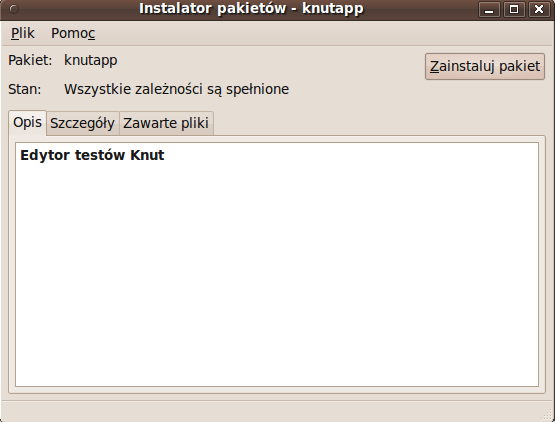
\includegraphics{Instalacja.png}
\end{quote}

Należy kliknąć na przycisk ``Zainstaluj pakiet'' i wprowadzić hasło administratora. Po chwili pojawi się komunikat o zakończonej istalacji. Program Knut będzie widoczny w menu systemu (Programy -\textgreater{} Edukacja -\textgreater{} Edytor testów Knut).
\begin{quote}

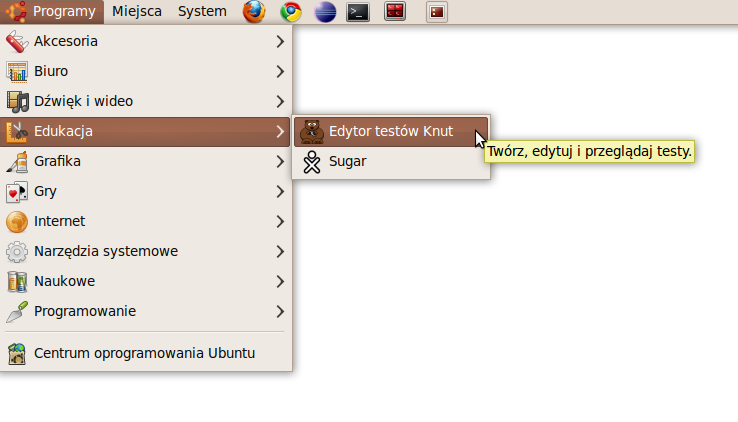
\includegraphics{MenuPoInstalacji.png}
\end{quote}


\section{Usunięcie programu}
\label{index:usuniecie-programu}\label{index:id4}
Aby usunąć program należy uruchomić komendę \code{sudo apt-get remove knutapp} w terminalu i wprowadzić hasło administratora. Polecenie to usunie wszystkie pliki programu oprócz testów i ustawień użytkownika, które znajdują sie na dysku twardym w katalogu \code{katalog\_domowy/.knutapp}. Można bezpiecznie usunąć zawartość tego katalogu jeśli nie zamierzamy korzystać z aplikacji.


\chapter{Tworzenie i edycja testu}
\label{index:tworzenie-i-edycja-testu}\label{index:tworzenie-edycja}
Aby utworzyć nowy test należy wybrać z menu okna programu \code{Test} a następnie \code{Nowy} lub użyć skrótu klawiaturowego \code{Ctrl + N}. Pojawi się wtedy okno właściwości testu.
\begin{quote}

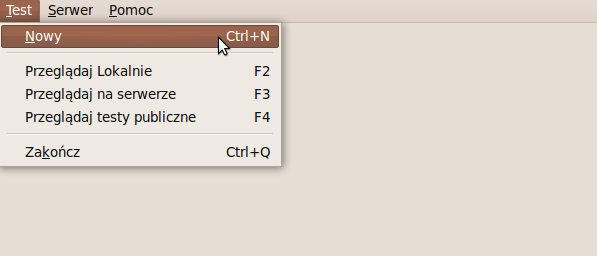
\includegraphics{NowyTest.png}
\end{quote}


\section{Właściwości testu}
\label{index:id5}\label{index:wlasciwosci-testu}\begin{description}
\item[{Właściwości testu:}] \leavevmode\begin{itemize}
\item {} 
opisują test

\item {} 
pomogają go odnaleźć

\item {} 
zawierają instrukcje dla uczniów

\item {} 
mogą zawierać hasło zabezpieczające przed nieupoważnionym pobraniem (np. nauczyciel podaje hasło w klasie i wszyscy uczniowie mogą równocześnie pobrać test).

\end{itemize}

\item[{Okno edycji właściwości * \emph{Założenie konta i konfiguracja ustawień serwera}}] \leavevmode\begin{itemize}
\item {} 
\emph{Zarządzanie testami na serwerze (zdalnie)}

\item {} 
\emph{Zarządzanie wynikami i odpowiedziami} testu

\end{itemize}

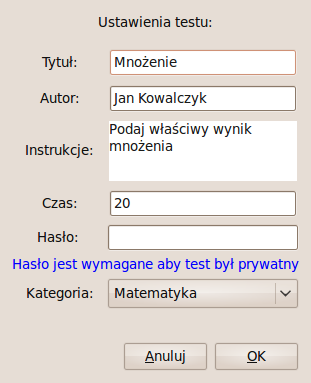
\includegraphics{WlasciwosciTestu.png}

\end{description}

Okno edycji właściwości testu pojawia się zawsze przy tworzeniu nowego testu, można również zmienić je wywołać po zapisaniu testu.

Wszystkie pola oprócz hasła sa wymagane. Jeśli hasło jest pozostawione puste, test będzie publiczny i każdy będzie mógł go pobrać i rozwiązać. W przeciwnym wypadku uczeń zostanie poproszony o hasło przed pobraniem testu.

Pozostałe pola używane są do identyfikacji testu i wyjaśnienia zdjącemu zasady testu.
Po uzupełnieniu właściwości testu program przechodzi do edycji testu (jeśli tworzymy nowy test)


\section{Edycja pytań}
\label{index:id6}\label{index:edycja-pytan}
Ekran edycji pytań wyświetla się po uzupełnieniu właściwości testu lub po rozpoczęciu edycji testu już istniejącego.

Ekran edycji pytań
\begin{quote}

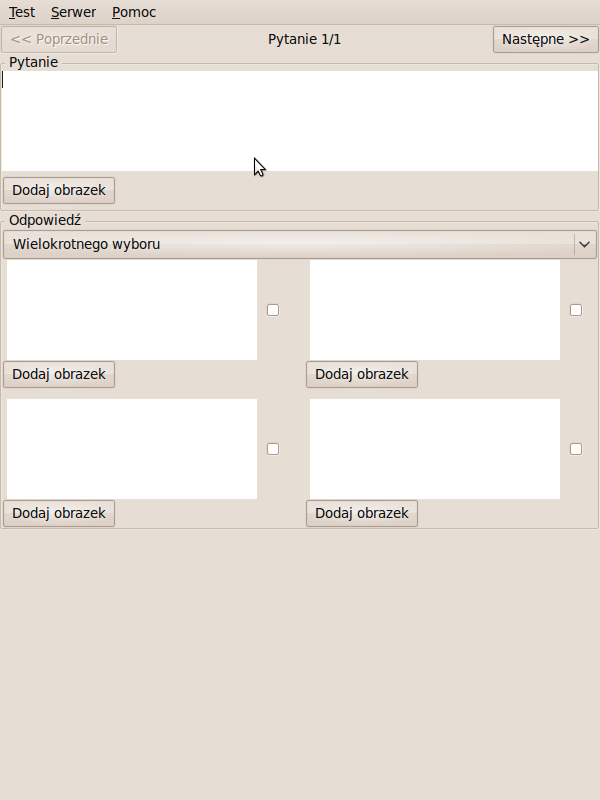
\includegraphics{OknoEdycjiPytania.png}
\end{quote}
\begin{description}
\item[{Ekran edycji pytania składa się z 3 części:}] \leavevmode\begin{itemize}
\item {} 
sekcji nawigacji pomiędzy pytaniami z numerem akutalnego pytania i liczby wszystkich pytań oraz przycisków nawigacyjnych do zmiany pytania na poprzednie i następne

\item {} 
sekcji pytania z polem tesktowym i możliwościa dodania obrazka

\item {} 
sekcji wyboru typu odpowiedzi i pól odpowiedzi

\end{itemize}

\item[{Program pozwala na tworzenie pytań:}] \leavevmode\begin{itemize}
\item {} 
jednokrotnego wyboru

\item {} 
wielkrotnego wyboru

\item {} 
prawda/fałsz

\end{itemize}

\end{description}

Pytanie jak i odpowiedzi mogą zawierać obrazek. Po kliknięciu w przycisk ``Dodaj obrazek'' pojawia się okno dialogowe pozwalające na wybór pliku graficznego w formacie png/jpeg/gif.


\section{Zapisywanie testu i ponowna edycja}
\label{index:zapisywanie-testu}\label{index:zapisywanie-testu-i-ponowna-edycja}
Zapisywanie poszczególnych pytań następuje po przejściu na następne/poprzednie pytanie. Po uzupełnieniu wszystkich pól pytania i naciścnięciu przycisku `Następne' lub `Poprzednie' program zaspiuje pytanie i przechodzi do pytania w wybranym kierunku.

Po przygotowaniu pytań test pojawi się na liście testów w bazie lokalnej. Funkcjonalność ta jest opisana w części XXX


\chapter{Zarządzanie testami, komunikacja z serwerem}
\label{index:zarzadzanie-testami}\label{index:zarzadzanie-testami-komunikacja-z-serwerem}
Po utworzeniu testy znajdują sie na komputerze użytkownika. Udostępnienie testu dla innych użytkowników edytora testów i uczniów odbywa się pośrednictwem serwera. Serwerem może być dowolny komputer w sieci z zainstalowanym kodem serwera dostępnym na knutest.org.
W tej części podręcznika użytkownika opisane jest zarządzanie testami i odpowiedziami uczniów.


\section{Zarządzanie zapisanymi testami}
\label{index:zarzadzanie-zapisanymi-testami}\label{index:zarzadzanie-zapisanymi}
Wyświetlenie testów dostępnych na dysku uzyskujemy przez wybranie z menu okna programu \code{Test} a następnie \code{Przeglądaj Lokalnie} lub użyć skrótu klawiaturowego \code{F2}
\begin{quote}

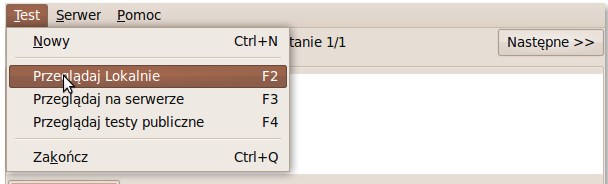
\includegraphics{PrzegladajLokalnie.png}
\end{quote}

Test będące aktualnie na dysku wyświetlane są w formie tabeli.
\begin{quote}

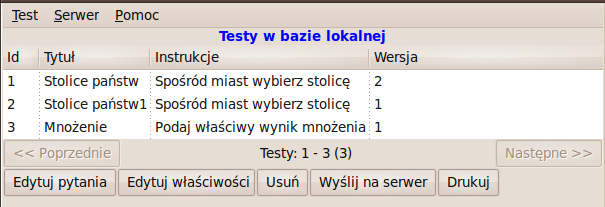
\includegraphics{TestyLokalnie.png}
\end{quote}

W pierwszej kolumnie znajduje się id testu, jest to numer porządkowy z bazy danych.

W kolejnych dwóch kolumnach jest tytuł i instrukcje testu podane w oknie edycji właściwości testu.

Ostatnia kolumna zawiera wersję testu. Kolejny numer wersji testu jest przydzielany po każdej edycji. Test nowo utworzony ma wersje 1. Jeśli edytujemy jego pytania raz, wersja zmieni się na 2. Wersja przydzielana jest przez program i użytkownik nie ma możliwości jej zmiany.
\begin{description}
\item[{Okno przeglądania testów ma dodatkowo przyciski pozwalające na manipulację zapisanymi testami. Są to kolejno:}] \leavevmode\begin{itemize}
\item {} 
\code{Edytuj pytania} - otwiera pytania wybranego testu (otwiera okno edycji pytań na pierwszym pytaniu)

\item {} 
\code{Edytuj właściwości} - otwiera okno edycji właściwości wybranego testu

\item {} 
\code{Usuń} - usuwa wybrany test z dysku, nie możliwości odzyskania usuniętego testu

\item {} 
\code{Wyślij na serwer} - wysyła test na serwer przez co umożliwia innym użytkownikom pobranie testu (więcej na ten temat w kolejnych rozdziałach)

\item {} 
\code{Drukuj} - otwiera okno menedżera drukowania testu

\end{itemize}

\end{description}


\section{Założenie konta i konfiguracja ustawień serwera}
\label{index:zalozenie-konta-i-konfiguracja-ustawien-serwera}\label{index:zalozenie-konta}
Do udostępniania testów wymagane jest konto na serwerze i odpowiednia konfiguracja edytora testów.

Istnieje możliwość założenia konta na knutest.org, w tym celu należy napisać e-mail na adres \href{mailto:wiktor.idzikowski@gmail.com}{wiktor.idzikowski@gmail.com}. Administrator serwera przydzieli nam nazwę użytkownika i hasło. Dane te należy wprowadzić do edytora testów.

W celu wprowadzenia ustawień serwera należy wybrać z menu okna programu \code{Serwer} a następnie \code{Preferencje} lub użyć skrótu klawiaturowego \code{F5}. Pojawi się wtedy okno ustawień serwera.
\begin{quote}

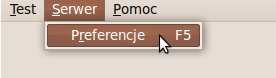
\includegraphics{UstawieniaSerwera.png}
\end{quote}

Pojawi się wtedy okno ustawień serwera.
\begin{quote}

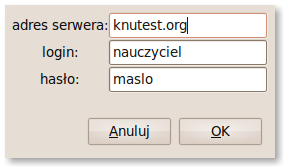
\includegraphics{OknoUstawienSerwera.png}
\end{quote}

Do komunikacji z serwerem wymagane są:
\begin{itemize}
\item {} 
Adres serwera - adres serwera w sieci bez http i www np. \code{knutest.org}

\item {} 
Login - podany przez administratora serwera, np. \code{jankowalski}

\item {} 
Hasło - podane przez administratora serwera, np. \code{maslo}

\end{itemize}

Wszystkie pola są wymagane do udostępniania testów.

Kolejne rozdziały opisują funkcje edytora testów wymagające poprawnych ustawień serwera.


\section{Zarządzanie testami na serwerze}
\label{index:id7}\label{index:zarzadzanie-testami-na-serwerze}
Edytor testów pozwala na współdzielenie testów z uczniami i innymi użytkownikami programu. Przeglądanie testów dostępnych na serwerze uzyskuję się poprzez wybranie z menu okna programu \code{Test} a następnie \code{Preferencje} lub użycie skrótu klawiaturowego \code{F3}
\begin{quote}

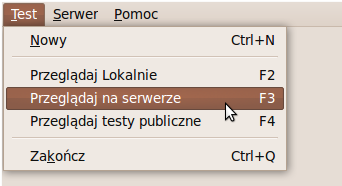
\includegraphics{PrzegladajSerwer.png}
\end{quote}

W rezultacie pojawi się lista dostępnych testów lub komunikat o braku testów na serwerze.

Test dostępne na serwerze wyświetlane są w formie tabeli.
\begin{quote}

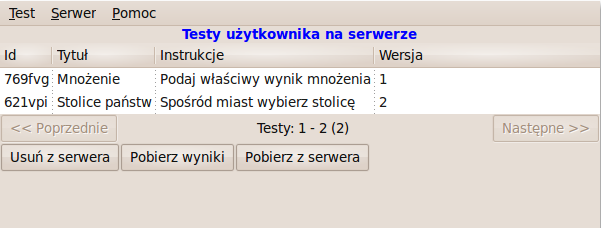
\includegraphics{PrzegladajNaSerwerze.png}
\end{quote}
\begin{description}
\item[{Okno przegladania testów zawiera 4 kolumny:}] \leavevmode\begin{itemize}
\item {} 
\code{Id} - unikalne id testu, przydatne do odnalezienia i identyfikacji testu

\item {} 
\code{Tytuł} - tytuł testu

\item {} 
\code{Instrukcje} - intrukcje przydatne przy rozwiązywaniu testu

\item {} 
\code{Wersja} - wersja testu

\end{itemize}

\item[{Okno przeglądania testów na serwerze ma dodatkowo przyciski pozwalające na manipulację testami. Są to kolejno:}] \leavevmode\begin{itemize}
\item {} 
\code{Usuń z serwera} - usuwa test z serwera

\item {} 
\code{Pobierz wyniki} - pobiera wyniki uczniów, którzy rozwiązywali test

\item {} 
\code{Pobierz z serwera} - pobiera test z serwera. Pobrany test będzie dostępny do edycji i pojawi się na liście testów lokalnych.

\end{itemize}

\end{description}


\section{Zarządzanie wynikami i odpowiedziami}
\label{index:zarzadzanie-wynikami-i-odpowiedziami}\label{index:zarzadzanie-wynikami}
Program umożliwia przeglądanie wyników i poszczególnych odpowiedzi uczniów. Odpowiedzi uczniów zapisywane są na serwerze i są dostępne dla osoby, która ułożyła dany test. Aby przejść do ekranu z wynikami należy na ekranie przeglądnia testów wybrać \code{Pobierz wyniki}.

Wyniki ucznia wyświetlane są w formie tabeli.
\begin{quote}

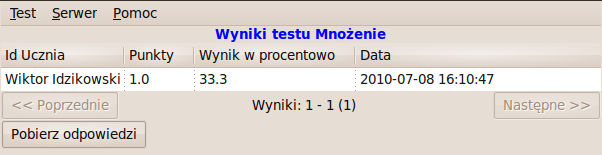
\includegraphics{WynikiUcznia.png}
\end{quote}

Okno wyników zawiera 4 kolumny:
\begin{itemize}
\item {} 
\code{Id Ucznia} - identyfikator ucznia

\item {} 
\code{Punkty} - wynik testu wyrażony w punktach

\item {} 
\code{Wynik procentowo} - wynik testu wyrażony procentowo

\item {} 
\code{Data} - data odesłania wyników

\end{itemize}

Istnieje możliwość zobaczenia odpowiedzi ucznia na poszczególne pytania. W tym celu należy kliknąć na wybrany wynik i następnie na przycisk \code{Pobierz odpowiedzi}. Pojawi się wtedy lista pytań i udzielonych odpowiedzi.

Ekran odpowiedzi ucznia na poszczególne pytania .
\begin{quote}

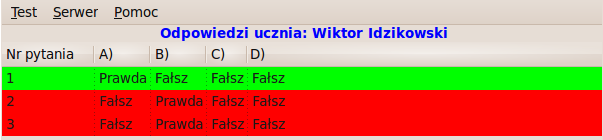
\includegraphics{OdpowiedziUcznia.png}
\end{quote}



\renewcommand{\indexname}{Indeks}
\printindex
\end{document}
